\documentclass[12pt]{article}

\usepackage{booktabs}% http://ctan.org/pkg/booktabs
\usepackage[utf8]{inputenc}
\usepackage{changepage}
\usepackage{pgfplots}
\usepackage{amssymb}
\usepackage{xcolor}
\usepackage{hyperref}
\usepackage{listings}
\usepackage[T1]{fontenc}
\usepackage[utf8]{inputenc}
\usepackage{adjustbox}
\usepackage{amsmath}
\usepackage{mathtools}
\usepackage{biblatex}
\usepackage{float}
\lstset{
  language=Python,
  numbers=left,
  numberstyle=\tiny,
  stepnumber=1,
  numbersep=5pt,
  tabsize=4,
  basicstyle=\ttfamily,
  columns=fullflexible,
  keepspaces,
}
\hypersetup{
    colorlinks,
    citecolor=black,
    filecolor=black,
    linkcolor=black,
    urlcolor=black
}

% Set page size and margins
% Replace `letterpaper' with `a4paper' for UK/EU standard size
\usepackage[letterpaper,top=2cm,bottom=2cm,left=3cm,right=3cm,marginparwidth=1.75cm]{geometry}

% Useful packages
\usepackage{amsmath}
\usepackage{mathtools}
\usepackage{graphicx}
\newenvironment{para}{\begin{adjustwidth}{13mm}{}}{\end{adjustwidth}}

\newcommand\tab[1][1cm]{\hspace*{#1}}

\newcommand{\tabitem}{\llap{\textbullet}}
\newcommand{\Hsquare}{%
\text{\fboxsep=-.2pt\fbox{\rule{0pt}{1ex}\rule{1ex}{0pt}}}%
}

\newtheorem{Definizione}{Definizione}[subsection]
\newtheorem{Lemma}{Lemma}[subsection]
\newtheorem{Teorema/Definizione}{Teorema/Definizione}[subsection]
\newtheorem{Corollario}{Corollario}[subsection]
\newtheorem{Teorema}{Teorema}[subsection]
\newtheorem{Proposizione}{Proposizione}[subsection]
\newtheorem{Notazione}{Notazione}[subsection]
\newtheorem{Commento}{Commento}[subsection]
\newtheorem{Dimostrazione}{Dimostrazione}[subsection]
\newtheorem{Osservazione}{Osservazione}[subsection]
\newtheorem{Nota}{Nota}[subsection]

\title{RSO: Reti}
\author{spitfire}
\date{A.A. 2024-2025}
\begin{document}
\begin{figure}
    \centering
    
\includegraphics[width=0.35\textwidth]{Images/Logo scienze bicocca.png}
\end{figure}

\vspace{10cm}
\date{A.A. 2024-2025}


\maketitle

\newpage

\tableofcontents
\newpage
\section{Introduzione}
Se vogliamo dare una visione "d'insieme" di internet possiamo pensarlo come formato dalle
seguenti componenti:
\begin{itemize}
    \item Miliardi di \textbf{calcolatori} connessi:
    \begin{itemize}
        \item \textbf{Hosts}: dispositivi di computazione e sistemi periferici
        \item Sono sistemi che eseguono \textbf{applicazioni di rete} al "confine" della rete
    \end{itemize}
    \item \textbf{Packet switches}: inoltrano i pacchetti ("pezzi" di dati) tra diversi nodi di rete
    \begin{itemize}
        \item Router, switches, ...
        \item Internet è una \textbf{rete a commutazione di pacchetto}
    \end{itemize}
    \item \textbf{Communication links}: I collegamenti fra i veri nodi della rede
    \begin{itemize}
        \item Fibra, rame, radio, satellite...
        \item \textbf{Transmission rate}: capacità, in termini di bit/s, che il canale può supportare ("larghezza di banda").
    \end{itemize} 
    \item \textbf{Networks}: Collezioni di dispositivi, router, switches e links gestiti \textbf{tutti da una stessa organizzazione}
    \begin{itemize}
        \item Reti residenziali, enterprise ecc... vengono dette solitamente \textbf{reti di accesso}, perché sono quelle reti che raccolgono il traffico
        dagli utenti per mandarlo in rete o viceversa.
    \end{itemize}
\end{itemize}
\begin{center}
    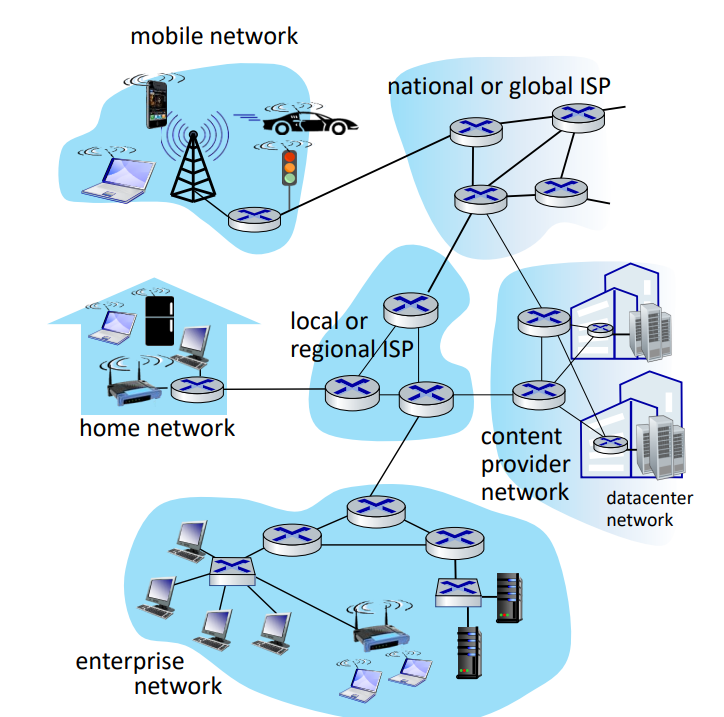
\includegraphics[width = 0.70\linewidth]{Images/1.PNG}
\end{center}
Internet è fisicamente una \textbf{rete connessa}, tuttavia vi sono dei sistemi che permettono di filtrare il traffico (firewall ecc...) per impedire che
ogni nodo della rete sia accessibile da un qualsiasi altro nodo. Internet è quindi una \textbf{rete di reti} che interconnette le reti
degli \textbf{Internet Service Providers} (ISP), cioè quelle entità che forniscono servizi di connettività. Il funzionamento della rete internet è governato
dai \textbf{protocolli di comunicazione}:
\begin{itemize}
    \item Controllano il modo in cui avviene l'invio e il ricevimento dei messaggi
    \item Esempi sono i protocolli HTTP (web), TCP, IP, WiFi, 4G, Ethernet ecc..
\end{itemize}
Protocolli di tipo diverso servono per \textbf{far comunicare dispositivi di tipo diverso}.
Poiché il contesto delle reti è quindi molto eterogeneo, il tutto riesce a funzionare grazie agli \textbf{standard}.
Esistono diversi enti di standardizzazione, tra cui citiamo:
\begin{itemize}
    \item \textbf{RFC}: Request for Comments, documenti
    \item \textbf{IETF}: Internet Engineering Task Force; rilascia le RFC
\end{itemize}
Il compito degli enti di standardizzazione è quello di rilasciare documenti che vanno a definire le caratteristiche
dei protocolli e delle architetture. Possiamo tuttavia vedere internet anche dal punto di vista dei \textbf{servizi}:
internet può essere quindi vista come una \textbf{infrastruttura che offre dei servizi di connettività alle applicazioni distribuite}.
Quindi, internet viene vista come una infrastruttura che \textbf{offre dei servizi di connettività tra nodi diversi}.
\begin{center}
    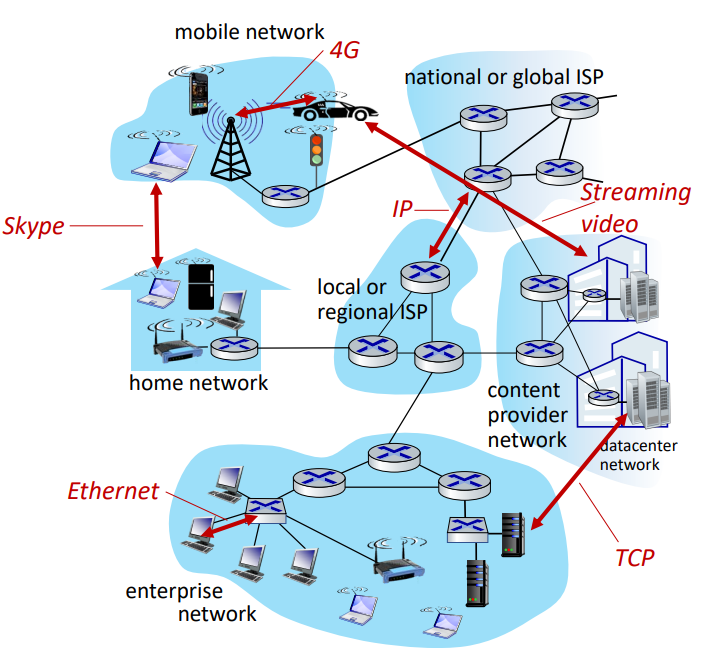
\includegraphics[width = 0.70\linewidth]{Images/2.PNG}
\end{center}
Abbiamo detto che la rete è governata da protocolli, ma \textbf{qual'è la definizione formale di protocollo?}
Una definizione formale può essere la seguente: i \textbf{protocolli} definiscono il \textbf{formato, l'ordine} dei \textbf{messaggi inviati e ricevuti} tra le entità di rete e le
\textbf{azioni intraprese} alla trasmissione e alla ricezione di un messaggio.
\begin{center}
    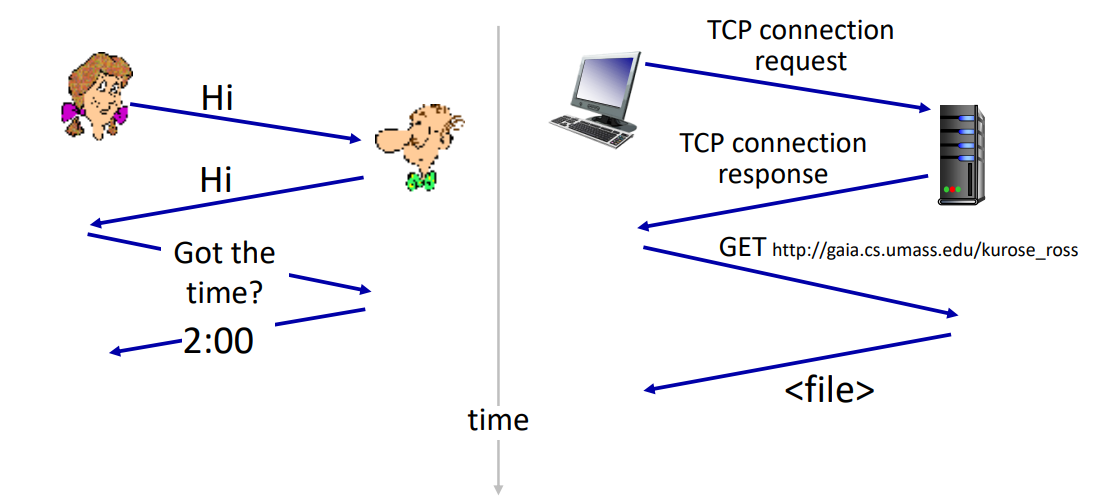
\includegraphics[width = 0.85\linewidth]{Images/3.PNG}
\end{center}
\subsection{Introduzione alla struttura di internet}
La struttura di alto livello di internet si può formalizzare nel seguente modo:
\begin{itemize}
    \item \textbf{Network edge}: il confine della rete, comprende
    \begin{itemize}
        \item \textbf{Hosts}: client e servers
        \item I servers sono spesso in \textbf{data centers}
    \end{itemize}
    È oggetto di dibattito se includere il confine della rete nella struttura di internet o meno; ciò nonostante, rimane comunque
    una componente fondamentale.
    \item \textbf{Access Networks}: Sono tutte quelle reti che servono a raccogliere il traffico generato e destinato per gli utenti.
    Sono quindi i \textbf{punti di accesso alla rete per gli utenti}. Esse possono essere \textbf{cablate oppure wireless}.
    \item \textbf{Network Core}: È l'insieme di tutte quelle reti che sono composte da router interconnessi che permettono di realizzare il concetto di \textbf{rete di reti}.
    Il suo compito è quello di \textbf{connettere le reti di accesso fra di loro} e comprendono tutte quelle reti che, su larga scala, \textbf{permettono il funzionamento di internet}.
\end{itemize}
Ogni componente della struttura di internet viene detto \textbf{segmento}.
\subsubsection{Network Edge}
Il confine della rete è \textbf{popolato dagli host}. Il suo compito principale è quello di inviare i \textbf{pacchetti}
generati dagli host (e quindi dagli utenti). Una visione ad alto livello di questo procedimento è:
\begin{itemize}
    \item Il \textbf{messaggio applicativo} viene generato dall'host
    \item Esso viene \textbf{spezzettato in pezzetti}, chiamati \textbf{pacchetti}, di lunghezza $L$ bits (questa cosa non è sempre vera: ci sono casi in cui i pacchetti hanno lunghezza variabile).
    Ognuno di questi pacchetti presenta una \textbf{intestazione}, cioè un determinato numero di bit che servono per permettere il funzionamento dei protocolli in rete
    \item Una volta generati i pacchetti, essi vengono trasmessi alla rete d'accesso ad un \textbf{tasso di trasmissione} (transmission rate) $R$, il quale è condizionato dalla \textbf{capacità di trasmissione del collegamento}
\end{itemize}
\begin{center}
    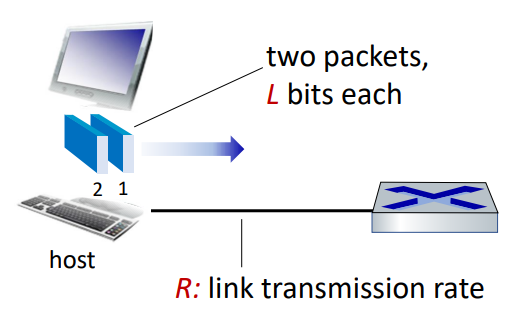
\includegraphics[width = 0.50\linewidth]{Images/4.PNG}
\end{center}
Ogni volta che invio un pacchetto in rete, ho un \textbf{ritardo di trasmissione}, il quale è il tempo necessario per trasmettere un pacchetto di $L$ bit su un collegamento che
ha capacità di trasporto di $R$ bit/sec. Quindi:
$$\textrm{packet transmission delay} = \frac{L \; (bits)}{R \; (bits/sec)}$$
\subsubsection{Access Networks}
Come facciamo a \textbf{connettere gli host a "internet"}? Il compito di effettuare questa connessione è delle
reti di accesso. Esse possono essere:
\begin{itemize}
    \item Reti di accesso \textbf{residenziali}
    \item Reti di accesso \textbf{istituzionali}
    \item Reti di accesso \textbf{mobili}
\end{itemize}
\subsubsection{Network Core}
La Network Core è un insieme di \textbf{maglie di rete interconnesse}, le quali sono fondamentali per effettuare le
operazioni di commutazione dei pacchetti. Esse garantiscono che i pacchetti possano essere trasmessi da un router verso l'altro
attraverso dei collegamenti da una sorgente a una destinazione.
Le reti di core presentano due \textbf{funzionalità fondamentali}:
per spiegarle, dobbiamo prima capire \textbf{come funziona un router}: esso possiede al suo interno una tabella chiamata
\textbf{tabella di inoltro} (forwarding table), che indica verso quale collegamento un pacchetto deve essere instradato in base al valore
della sua intestazione (che quindi contiene, in termini generici, a chi deve essere recapitato questo pacchetto).
L'operazione di \textbf{inoltro} (o \textbf{commutazione di pacchetto}) quindi consiste nell'invio sulla connessione corretta del pacchetto in arrivo (questa operazione viene anche detta \textbf{switching}).
L'inoltro ha \textbf{valenza locale}: ogni router prende in considerazione solo la propria tabella di inoltro locale per decidere dove inoltrare un pacchetto.
Tuttavia, questa operazione non basta per garantire che io possa raggiungere la destinazione corretta; per garantirlo dobbiamo effettuare un'altra operazione che prende il nome di
\textbf{instradamento} (routing). Il routing è un'operazione \textbf{globale} che è utilizzata per determinare \textbf{quale percorso, fra sorgente e destinazione, devono attraversare i pacchetti}.
Ogni singolo router esegui quindi dei \textbf{protocolli} e degli \textbf{algoritmi di routing distribuiti} che hanno l'obbietto di \textbf{popolare le tabelle di inoltro} (viene effettuato tramite algoritmi su grafo).
Poiché gli algoritmi di routing sono \textbf{distribuiti}, essi richiedono lo \textbf{scambio di messaggi e la collaborazione tra i router}.
\begin{center}
    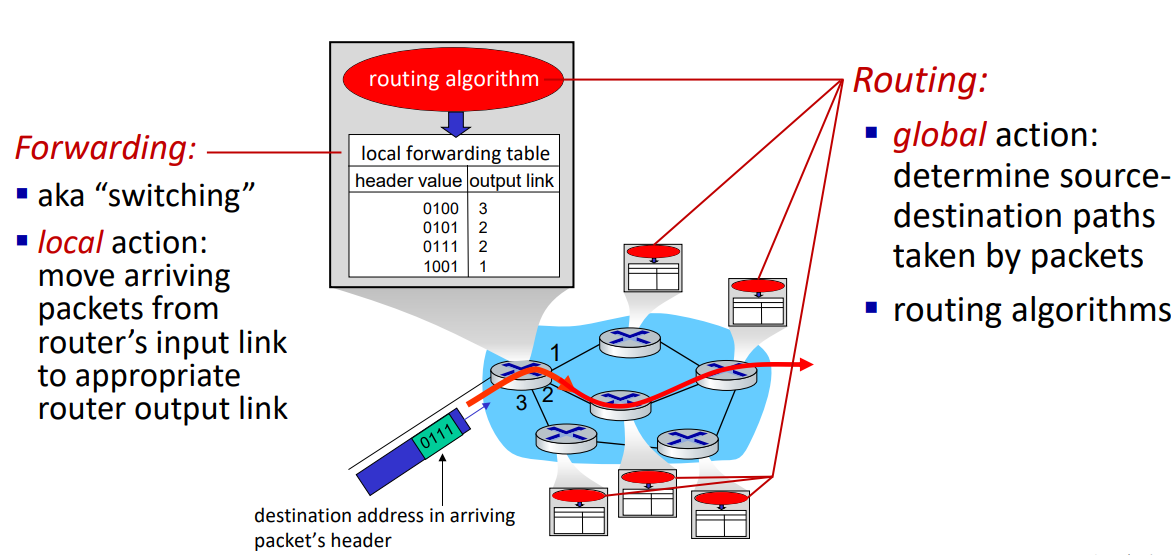
\includegraphics[width = 1\linewidth]{Images/5.PNG}
\end{center}
\subsection{Packet Switching: Store-and-Forward}
Nelle reti a commutazione di pacchetto, \textbf{ogni pacchetto ha vita propria}: una volta che il messaggio viene spezzettato in pacchetti, ognuno di esso
ha un ciclo di vita indipendente dagli altri. La modalità di trasmissione usata da tutte le reti a commutazione di pacchetto è quella del \textbf{store-and-forward}:
quando un pacchetto arriva ad un commutatore per essere commutato, esso deve \textbf{arrivate interamente prima di essere trasmesso al nodo successivo}. Tuttavia, si può pensare
di saltare questo passaggio e trasmettere direttamente ogni bit che arriva su un certo nodo al successivo. Perché non viene fatto nelle reti a commutazione di pacchetto? Il motivo risiede nelle \textbf{intestazioni dei pacchetti}:
infatti, è li che trovo \textbf{tutte le informazioni necessarie per gestire un pacchetto}, quindi devo aspettare che essa venga trasmessa per intero prima di procedere all'invio al nodo successivo.
\begin{center}
    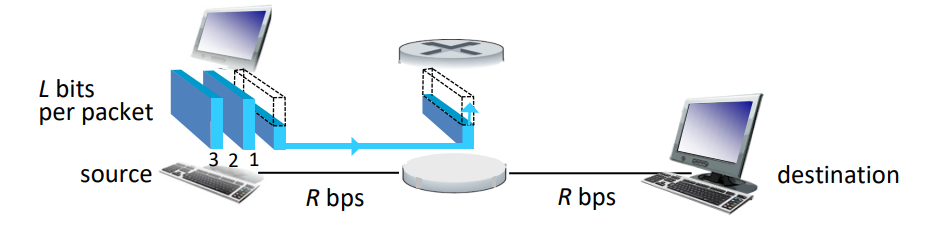
\includegraphics[width =1\linewidth]{Images/6.PNG}
\end{center}
\subsection{Packet-Switching: queuing}
Seppur Store-and-Forward semplifichi di molto la gestione delle reti, esso introduce una problematica che prende il nome di
\textbf{accodamento} (queueing). È una problematica che esiste in tutte le reti e si manifesta quando il \textbf{tasso di arrivo dei pacchetti è superiore al tasso di trasmissione in uscita}.
Nei router e negli switch, i pacchetti si accodano in aree di memoria apposite dette \textbf{buffer}; un pacchetto rimane nel buffer fino a quando non verrà trasmesso.
\begin{center}
    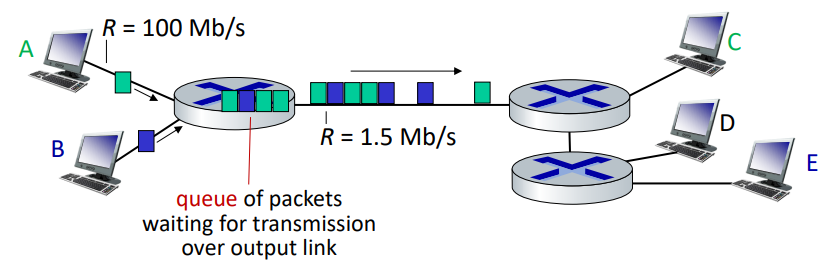
\includegraphics[width =0.90\linewidth]{Images/7.PNG}
\end{center}
Questa è una condizione che può accadere nelle reti a commutazione di pacchetto, tuttavia \textbf{non può essere una situazione sistematica}:
se si verificasse costantemente, la dimensione del buffer \textbf{crescerebbe costantemente} fino a raggiungere la massima dimensione possibile; da quel momento
in poi ogni pacchetto in arrivo porta a una condizione di \textbf{buffer overflow} e andrebbe perso. Quindi, quali sono i problemi che provoca l'accodamento?
\begin{itemize}
    \item \textbf{Buffer overflow} dei buffer dove vengono salvati i pacchetti ancora da trasmettere e susseguente perdita dei pacchetti in arrivo
    \item \textbf{Ritardo di accodamento} dato dall'attesa che il router trasmetta il pacchetto
\end{itemize}
\subsection{Circuit Switching}
La commutazione di pacchetto non è l'unico tipo di commutazione esistente; anzi essa storicamente è posteriore ad un'altro tipo di commutazione
che prende il nome di \textbf{commutazione a circuito}
\begin{center}
    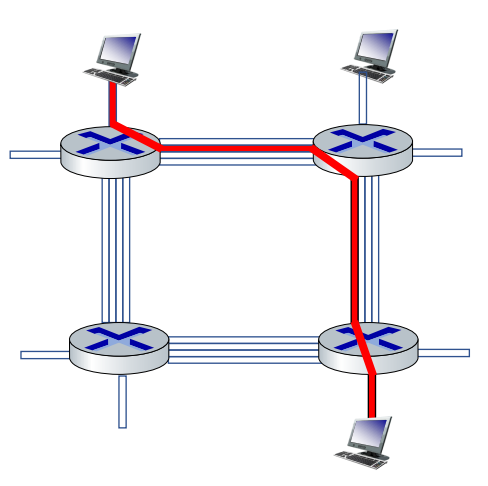
\includegraphics[width =0.45\linewidth]{Images/8.PNG}
\end{center}
Questo tipo di commutazione segue un principio diverso da quella a commutazione di pacchetto: l'elemento fondamentale di questo tipo di rete è il \textbf{circuito} (non esistono i pacchetti in questo tipo di rete).
Tra i vari \textbf{commutatori di circuito} si possono stabilire un certo numero di circuiti.
L'obbiettivo di questo tipo di commutazione è \textbf{destinare i circuiti alla comunicazione tra gli utenti della rete}.
Le risorse di un circuito vengono \textbf{assegnate in maniera esclusiva ad un host} e non possono essere condivise con altri host.
Il vantaggio di questo tipo di commutazione è \textbf{l'assenza di accodamento} data dal completo assegnamento delle risorse di un circuito
ad una sola comunicazione tra sorgente e destinazione.
Viene chiamato \textbf{circuito end-to-end} l'insieme di tutti i circuiti che vengono stabiliti tra sorgente e destinazione.
Uno svantaggio di questo tipo di commutazione è la \textbf{necessità di una fase di setup} in cui vengono allocate le risorse dei circuiti per andare a creare
il circuito end-to-end.
\subsubsection{Packet Switching vs Circuit Switching}
In una commutazione di circuito, le risorse vengono allocate solamente alla comunicazione tra sorgente e destinazione e non esistono
problemi di accodamento. Tuttavia, l'utilizzo delle risorse di rete in questo tipo di comunicazione risulta \textbf{subottimale} rispetto ad una
rete a commutazione di pacchetto. Facciamo un esempio:
\begin{center}
    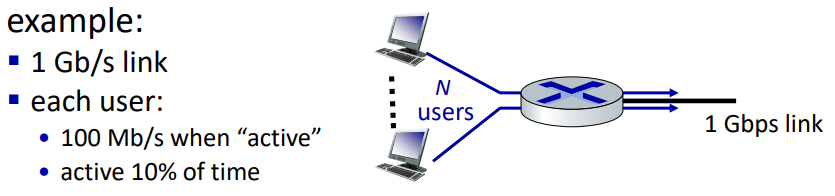
\includegraphics[width =0.75\linewidth]{Images/9.PNG}
\end{center}
\textbf{Domanda: quanti utenti, in queste condizioni, possono rispettivamente accomodare una rete a commutazione di circuito e una rete a commutazione di pacchetto?}
\begin{itemize}
    \item \textbf{Circuit-switching}: 10 utenti
    \item \textbf{Packet-switching}: con 35 utenti, la probabilità che più di 10 utenti siano attivi allo stesso tempo è minore di $0.0004$
\end{itemize}
Quindi una rete a commutazione di pacchetto è sempre la scelta migliore?
\begin{itemize}
    \item Essa è ottima per un traffico di tipo \textbf{"bursty"} (a raffica), cioè in situazioni dove a volte ci sono dati da inviare, a volte no
    \item Permette la condivisione delle risorse di rete
    \item Non richiede setup
\end{itemize}
Tuttavia, se si creano condizioni sfavorevoli, si vanno a creare delle \textbf{situazione di congestione eccessiva della rete}, andando a creare situazioni
di ritardo nella trasmissione dei pacchetti e di buffer overflow. Si rendono quindi necessari \textbf{protocolli di trasmissione affidabili} e meccanismi di \textbf{controllo della congestione}.
È però possibile, visti i vantaggi delle reti a commutazione di circuito, fornire lo stesso tipo di garanzia del servizio anche nelle reti a commutazione di pacchetto?
La risposta è si; esistono delle tecniche che permettono di \textbf{emulare la commutazione di circuito sulle reti a commutazione di pacchetto}, tuttavia sono casi parecchio difficili da gestire.
\subsection{Struttura di internet nel dettaglio}
Gli host sono connessi a internet tramite le \textbf{reti di accesso} fornite da ISPs.
Le reti di accesso devono per forza essere \textbf{interconnesse} per garantire che possa avvenire la comunicazione tra qualsiasi due host della rete (internet è una rete \textbf{connessa}, cioè ogni nodo è raggiungibile da tutti gli altri nodi).
Il risultato dell'evoluzione di internet è una \textbf{struttura gerarchica}; questa evoluzione, tuttavia, non è stata guidata da \textbf{necessità di tipo tecnico} ma di tipo \textbf{economico e politico}.
Vediamo quindi la struttura di internet passo passo: al mondo abbiamo \textbf{milioni} di reti di accesso
\begin{center}
    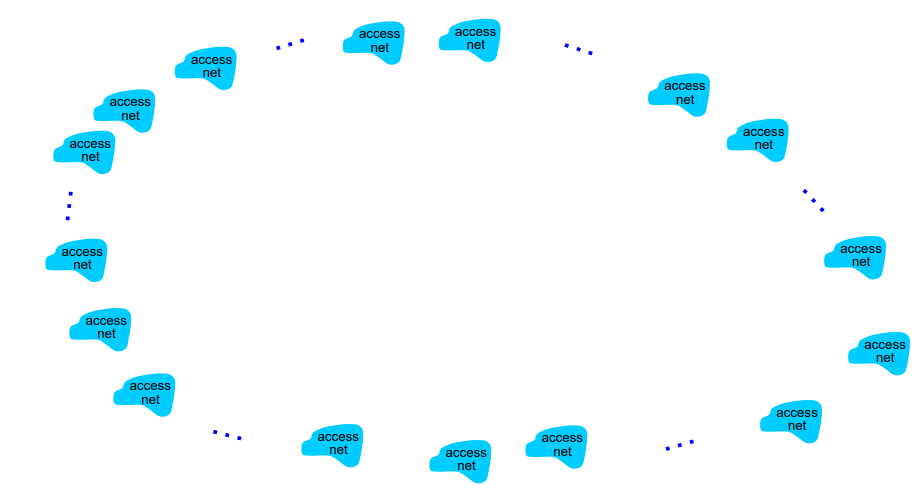
\includegraphics[width =0.85\linewidth]{Images/10.PNG}
\end{center}
L'idea più semplice per interconnetterle è \textbf{connettere ogni ISP agli altri in maniera diretta}, tuttavia...
\begin{center}
    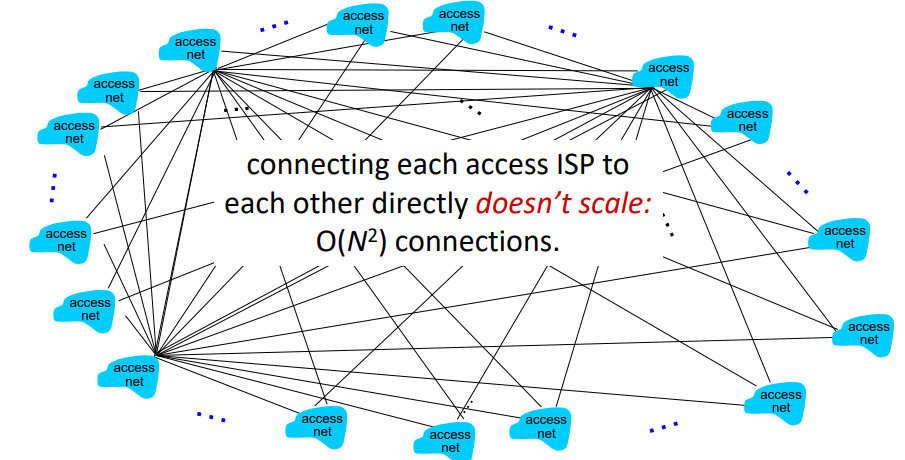
\includegraphics[width =0.85\linewidth]{Images/11.PNG}
\end{center}
Una soluzione alternativa è quella di avere un \textbf{ISP globale} (o di transito) con una rete geograficamente estesa in tutto il mondo, i cui router sono \textbf{interconnessi} e che fornisce connettività alle reti di accesso:
\begin{center}
    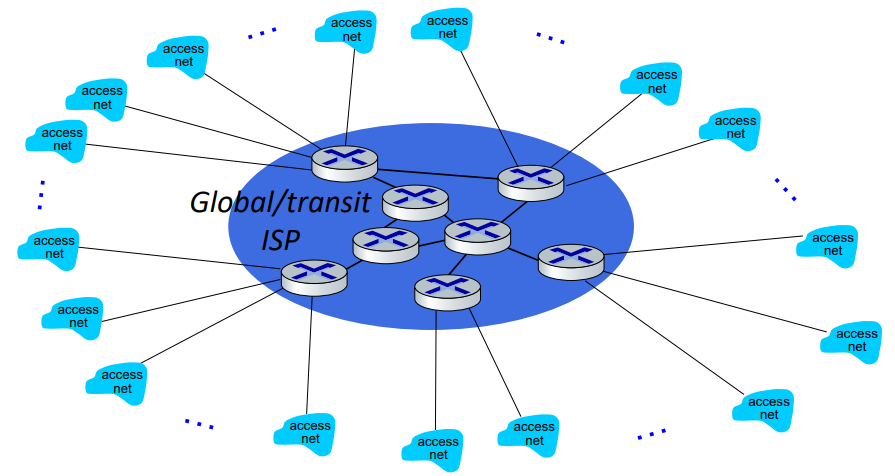
\includegraphics[width =0.85\linewidth]{Images/12.PNG}
\end{center}
Questo approccio tuttavia ha dei problemi:
\begin{itemize}
    \item Richiede una rete estesa \textbf{su tutto il globo}, in modo che possa servire ogni rete di accesso
    \item Richiede un accordo economico tra gli ISP locali e quello globale
    \item Perché ci si dovrebbe limitare ad un solo ISP globale? In effetti, ci potrebbe essere concorrenza fra essi
\end{itemize}
In virtù dell'ultimo punto sopra, si è andata a creare una situazione di questo tipo:
\begin{center}
    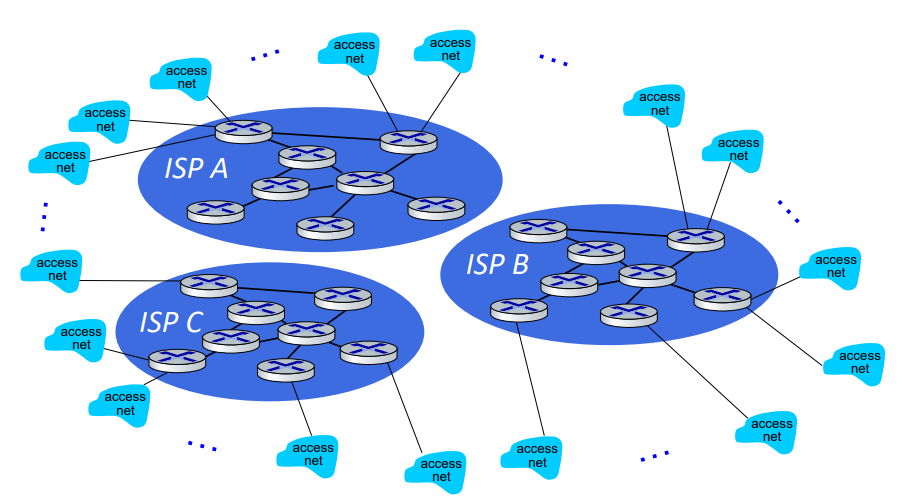
\includegraphics[width =0.85\linewidth]{Images/13.PNG}
\end{center}
si sono andati quindi a creare degli ISPs \textbf{geograficamente estesi} che coprono determinate aree del globo.
Questo genere di ISPs prendono il nome di \textbf{Tier 1 ISPs}.
A questo punto, gli ISPs globali devono creare dei \textbf{peering links} (chiamati così perché \textbf{non sono il frutto di un accordo economico ma di un accordo tra pari})
per creare un'interconnessione tra di loro:
\begin{center}
    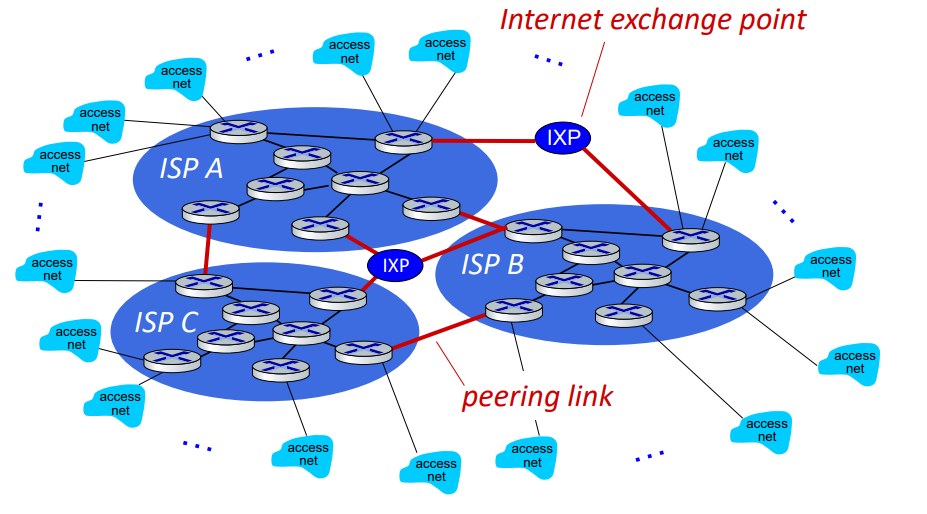
\includegraphics[width =0.85\linewidth]{Images/14.PNG}
\end{center}
Tuttavia, c'è anche un'altra possibilità, cioè quella di avere degli \textbf{Internet Exchange Points} (IXPs), i quali sono dei nodi a cui gli ISPs globali si connettono e che garantiscono
la connessione tra di essi. Tuttavia, tipicamente le reti di acceso non si \textbf{interfacciano direttamente con gli ISPs globali} ma passano tramite \textbf{ISPs regionali}, che hanno una diffusione
più capillare sul territorio. Altro tipo modo in cui le reti di accesso accedono agli ISPs globali è tramite \textbf{multi-homing}, cioè una rete di accesso potrebbe avere \textbf{più collegamenti verso un ISPs globale o regionale};
questo approccio garantisce \textbf{resilienza}
\begin{center}
    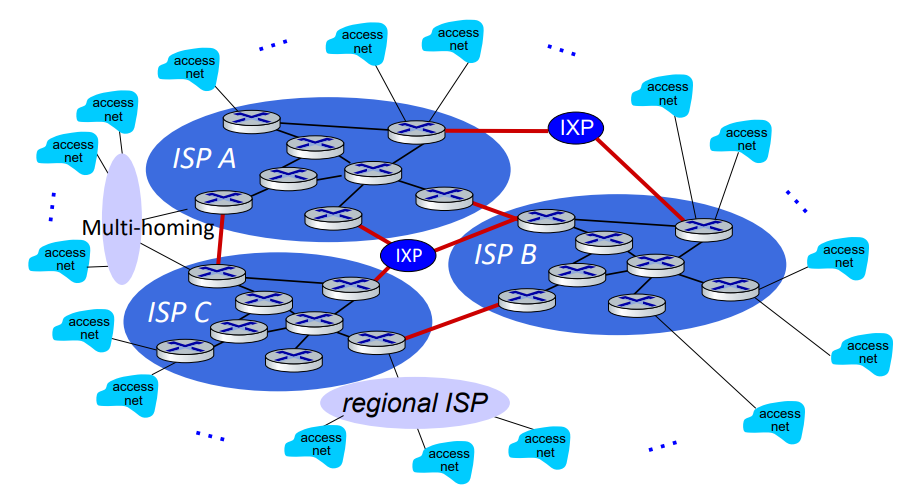
\includegraphics[width =0.85\linewidth]{Images/15.PNG}
\end{center}
Infine, abbiamo le \textbf{reti dei content provider}, che hanno lo scopo di \textbf{fornire contenuto agli utenti}. Per farlo, molto spesso, esse \textbf{bypassano gli ISPs globali} e si interfacciano
direttamente con le reti di accesso.
\begin{center}
    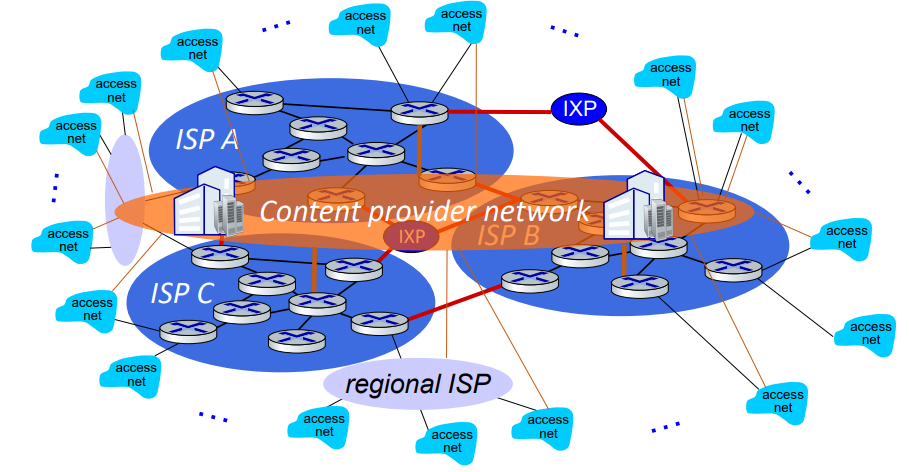
\includegraphics[width =0.85\linewidth]{Images/16.PNG}
\end{center}
Nulla però vieta alle reti dei content provider di accedere anche alle reti degli ISPs globali.
Diamo una versione più generale della gerarchia:
\begin{center}
    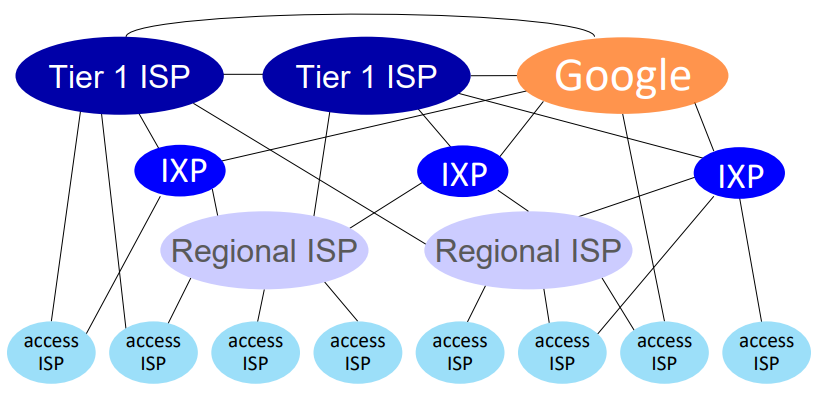
\includegraphics[width =0.85\linewidth]{Images/17.PNG}
\end{center}
Tuttavia, le connessioni possibili \textbf{possono anche non limitarsi a quelle mostrare in figura}.
\subsection{Metriche di performance nelle reti}
Il ritardo e la perdita sono due delle metriche fondamentali per capire la prestazione della rete.
Abbiamo già parlato di \textbf{ritardo di accodamento} e di \textbf{ritardo di trasmissione}, tuttavia essi sono
solo due dei tipi di ritardo che si possono verificare.
\begin{center}
    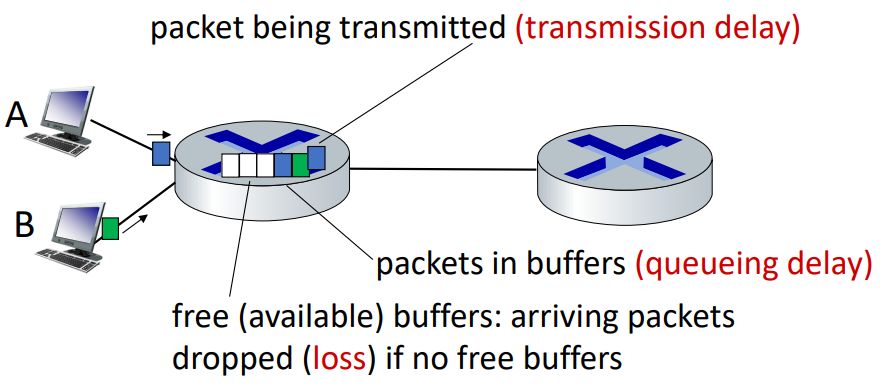
\includegraphics[width =0.70\linewidth]{Images/18.PNG}
\end{center}
Tuttavia ce ne sono delle altre, vediamole tutte: 
\begin{itemize}
    \item \textbf{Ritardo di elaborazione} ($d_{proc}$): quando un pacchetto arriva ad un nodo, devono essere effettuate delle operazioni fondamentali, per esempio \textbf{l'analisi della tabella di inoltro per capire su quale collegamento trasmettere il pacchetto} (lookup).
    Altra operazione è il \textbf{controllo dei bit di errore}: a volte, per colpa di distorsioni o "rumore" sul canale, certi bit di un pacchetto possono essere cambiati (da 0 a 1 e viceversa); il pacchetto quindi risulta malformato. Esistono meccanismi che permettono
    di \textbf{individuare se c'è stato un errore} (e anche di ricostruire il pacchetto originale). Questi metodi sono detti di \textbf{controllo e correzione dell'errore} e richiedono del tempo per essere eseguiti, tendenzialmente nell'ordine dei \textbf{microsecondi} ($10^-6 s$).
    \item \textbf{Ritardo di accodamento} ($d_{queue}$): è il tempo che il pacchetto attende per essere trasmesso. Dipende dal livello di congestione della rete. È tipicamente nell'ordine dei millisecondi
    \item \textbf{Ritardo di trasmissione} ($d_{trans}$): Se abbiamo un pacchetto di lunghezza $L$ che vogliamo trasferire su un collegamento con tasso di trasmissione $R$, allora il ritardo di trasmissione è dato da:
    $$d_{trans} = \frac{L}{R}$$
    \item \textbf{Ritardo di propagazione} ($d_{prop}$): Il ritardo di propagazione è il tempo che necessita un pacchetto per \textbf{propagarsi da un capo all'altro del collegamento}. Questo ritardo dipende dalla lunghezza del collegamento fisico $d$ (espressa in \textbf{metri} (m))
    e dalla \textbf{velocità di propagazione} $s$, che è nell'ordine di grandezza della \textbf{velocità della luce}: $\sim 2 \cdot 10^8 \; m/sec$, e si calcola nel seguente modo:
    $$d_{prop} = \frac{d}{s}$$
\end{itemize}
\begin{center}
    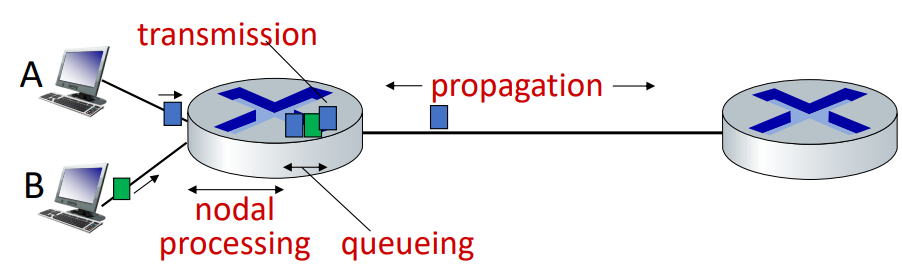
\includegraphics[width =0.70\linewidth]{Images/19.PNG}
\end{center}
Il \textbf{ritardo totale del nodo} (ritardo \textbf{end-to-end}) $d_{nodal}$ è calcolato come la somma di tutti ritardi visti sopra:
$$d_{nodal} = d_{proc} + d_{queue} + d_{trans} + d_{prop}$$
esso è uno delle \textbf{metriche più importanti} e mi permette di valutare le prestazioni della rete. Per calcolare il ritardo ent-to-end bisognerebbe anche tener conto dei \textbf{ritardi introdotti dai sistemi periferici},
che tuttavia non considereremo per questi appunti.
\subsubsection{Ritardo di accodamento e intensità di traffico}
Il ritardo di accodamento ha una caratteristica particolare: mentre tutti gli altri ritardi sono \textbf{analoghi} se considero lo stesso pacchetto trasmesso in due momenti diversi, \textbf{per il ritardo di accodamento non è così}.
Il ritardo di accodamento dipende dallo stato della rete durante la trasmissione. Questo ritardo di solito viene studiato tramite \textbf{metodi statistici}: in particolare, il ritardo di accodamento dipende da un valore che viene chiamato \textbf{intensità di traffico} ("traffic intensity"):
$$\frac{L \cdot \overline{a}}{R} = \frac{\textrm{tasso di arrivo dei pacchetti (bit/s)}}{\textrm{tasso di uscita dei pacchetti (bit/s)}}$$
Dove:
\begin{itemize}
    \item $\overline{a}$ è il \textbf{tasso di arrivo medio dei pacchetti} (pacchetti/s)
    \item $L$ è la \textbf{lunghezza} dei pacchetti (bit/packet)
    \item $R$ è la \textbf{larghezza di banda} del collegamento (bit/s)
\end{itemize}
L'intensità di traffico è \textbf{adimensionale} ed è una quantità non negativa:
\begin{itemize}
    \item Se l'intensità di traffico è \textbf{vicina a 0}, allora il ritardo di accodamento medio sarà piccolo
    \item Se l'intensità di traffico è \textbf{vicina a 1}, allora il ritardo di accodamento medio è grande
    \item Se l'intensità di traffico è \textbf{maggiore di 1}, allora il tasso di arrivo dei pacchetti \textbf{è troppo alto rispetto alla capacità della rete di smaltirli}, quindi il tempo di accodamento medio è \textbf{potenzialmente infinito}
\end{itemize}
\begin{center}
    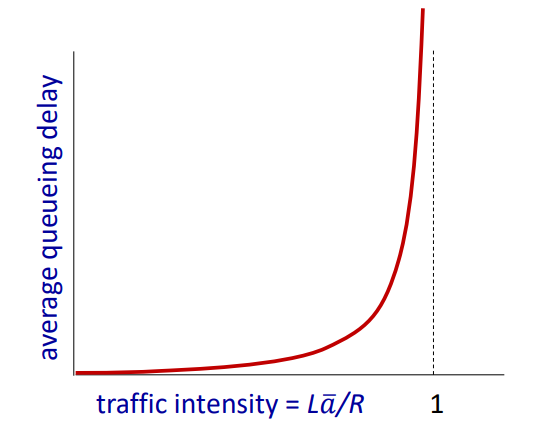
\includegraphics[width =0.50\linewidth]{Images/20.PNG}
\end{center}
\subsubsection{Perdita di pacchetti}
Un'altra metrica di performance fondamentale è la \textbf{perdita di pacchetti}; infatti, idealmente essa dovrebbe essere \textbf{nulla}.
La perdita di pacchetti si verifica quando si ha un buffer overflow sul buffer di accodamento di un nodo.
La perdita di pacchetti può essere mitigata tramite \textbf{meccanismi di ritrasmissione dei pacchetti} da parte del nodo sorgente (tuttavia non è obbligatorio che avvenga).
\begin{center}
    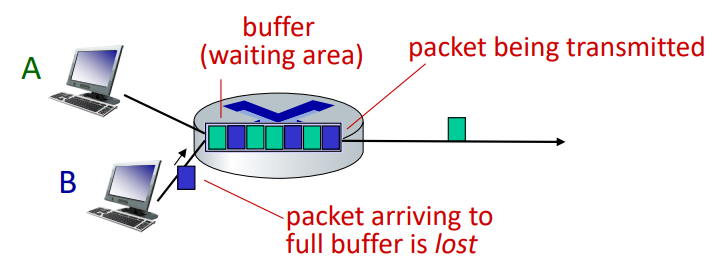
\includegraphics[width =0.70\linewidth]{Images/21.PNG}
\end{center}
Oltre alla perdita per accodamento, \textbf{i pacchetti possono essere scartati dai commutatori} se ci sono stati troppi errori durante la trasmissione oppure se non è previsto un meccanismo di correzione degli errori.
\subsubsection{Throughput}
Il \textbf{throughput} è il \textbf{tasso a cui i bits vengono inviati dal mittente al destinatario}; si calcola in bit/s e viene a volte chiamato \textbf{throughput end-to-end}.
Come si fa a calcolare il throughput?
\begin{itemize}
    \item \textbf{Throughput istantaneo}: tasso di invio \textbf{ad un certo punto nel tempo}
    \item \textbf{Throughput medio}: tasso di invio medio \textbf{su un lungo periodo di tempo}; si può ottenere facendo la media di tutti i valori istantanei o nel seguente modo: supponiamo di voler trasferire un file $F$ dal punto A al punto B; allora il throughput sarà la dimensione del file diviso il tempo che ha impiegato il file ad essere trasferito 
\end{itemize}
Il throughput è una metrica di prestazione "quanto bene" la rete sta andando nella comunicazione tra un mittente ed un destinatario.
\begin{center}
    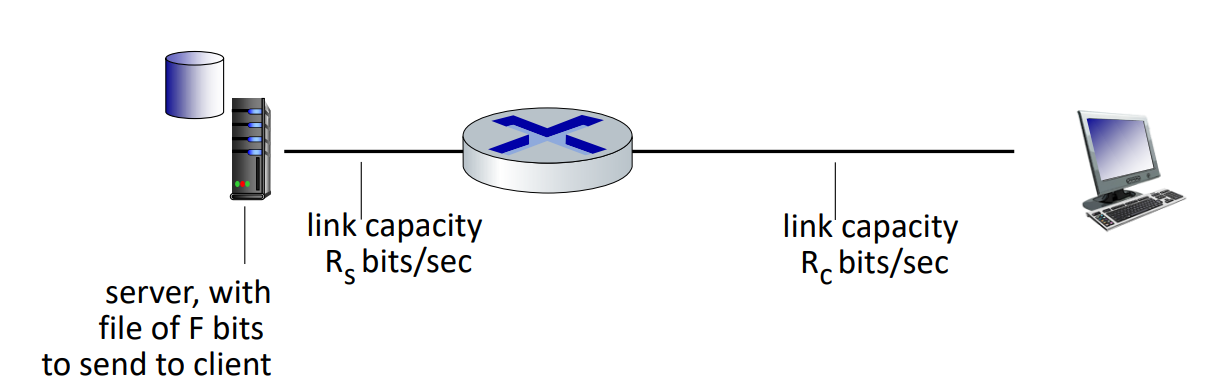
\includegraphics[width =1\linewidth]{Images/22.PNG}
\end{center}
Si possono verificare vari casi:
\begin{itemize}
    \item Se $R_s < R_c$ allora il throughput medio sarà $R_s$. In questo caso, \textbf{non si causerà mai accodamento nel commutatore}
    \item Se $R_s > R_c$ allora il throughput medio sarà $R_c$. In questo caso, potrebbe essere possibile che i \textbf{pacchetti si accodano nel commutatore}
\end{itemize}
In ogni caso, il throughput è vincolato dal collegamento con capacità minore, il quale prende il nome di \textbf{bottleneck link}. Vediamo questo ulteriore scenario:
supponiamo di avere 10 client e 10 server e che essi, per comunicare, passino attraverso un collegamento all'interno della network core con larghezza di banda $R$:
\begin{center}
    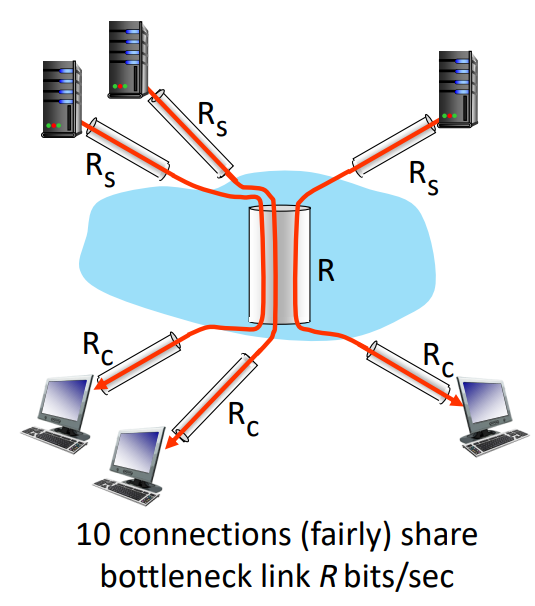
\includegraphics[width =0.40\linewidth]{Images/23.PNG}
\end{center}
In questo caso, il throughput end-to-end per connessione risulta il minimo tra $R_c, R_s,$ e $R/10$, cioè $min\{R_C, R_s, R/10\}$.
Nella pratica, tuttavia, la rete di core ha larghezze di banda \textbf{molto maggiori rispetto ai collegamenti degli hosts}, quindi $R/10$, il più delle volte, sarà comunque molto maggiore di $R_s$ e $R_c$.
Ciò significa che, molto spesso, il bottleneck è dato dai collegamenti di accesso.
\subsection{Strato protocollare e modelli di servizio}
Le reti sono dei sistemi molto complessi con diverse componenti che interagiscono fra loro
\begin{itemize}
    \item Hosts
    \item Routers
    \item Collegamenti di diverso tipo e scopo
    \item Applicazioni
    \item Protocolli
    \item Hardware e Software
\end{itemize}
C'è allora un modo intelligente per \textbf{strutturare e discutere le reti}?
Un modo è una \textbf{struttura a strati}, in cui ogni servizio viene implementato tramite \textbf{azioni interne allo strato} e ogni servizio fa affidamento ai servizi \textbf{appartenenti al livello sottostante per implementare le proprie operazioni e garantirne il funzionamento}.
Inoltre, i vari strati sono \textbf{indipendenti l'uno dall'altro}, nel senso che, in caso di modifiche a come vengono implementati i servizi in uno strato, gli altri strati \textbf{non vengono influenzati dalla modifica}.
L'approccio a strati quindi permette di approcciarsi alla modellazione e alla discussione di sistemi complessi:
\begin{itemize}
    \item La sua \textbf{struttura esplicita} permette l'identificazione e le \textbf{relazioni fra le varia componenti del sistema}. Crea inoltre un \textbf{modello di riferimento a strati} per la discussione
    \item Permette la \textbf{modularizzazione} del sistema e quindi rende più semplice l'aggiornamento e la manutenzione di questo
    \begin{itemize}
        \item I cambiamenti nell'implementazione dei servizi di uno strato sono \textbf{trasparenti al resto del sistema} e quindi non lo influenzano
    \end{itemize}
\end{itemize}
Ciò che è stato definito per internet prende il nome di \textbf{pila (o stack) protocollare di internet} e prevede l'esistenza di 5 diversi strati, numerati dal basso verso l'alto:
\begin{center}
    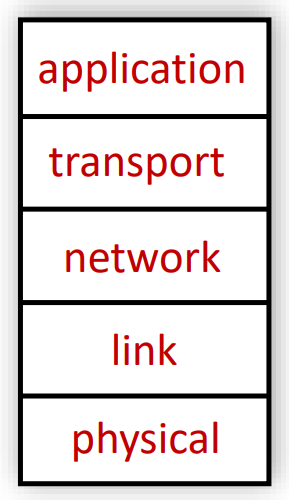
\includegraphics[width =0.15\linewidth]{Images/24.PNG}
\end{center}
Vediamoli nel dettaglio:
\begin{itemize}
    \item \textbf{LIVELLO 5: APPLICATIVO}: Tutti i protocolli volti al supporto alle applicazioni di rete (HTTP, SMTP, DNS ecc..)
    \item \textbf{LIVELLO 4: TRASPORTO}: Ha il compito di effettuare un trasferimento di dati tra macchine che si trovano su reti differenti. Esempio di protocolli a questo livello sono TCP e UDP
    \item \textbf{LIVELLO 3: RETE}: Offre il servizio fondamentale di \textbf{instradamento} tra sorgente e destinazione. Protocollo fondamentale a questo livello è \textbf{Internet Protocol} (IP)
    \item \textbf{LIVELLO 2: COLLEGAMENTO}: Ha il compito di trasferire i dati tra \textbf{due entità di rete adiacenti}, cioè su un collegamento. Protocolli a questo livello sono, per esempio, Ethernet e 802.11(WiFi).
    \item \textbf{LIVELLO 1: FISICO}: Trasporto fisico dei bit su un cavo (o canale radio)
\end{itemize}
\subsubsection{Servizi, Stratificazione e Incapsulamento}
Come si può andare ad implementare i vari protocolli che garantiscono il funzionamento dei servizi ad ogni livello?
Un concetto fondamentale da introdurre a questo scopo è quello dell'\textbf{incapsulamento}: le applicazioni si devono
scambiare messaggi per realizzare i propri servizi, e per farlo devono basarsi sui servizi offerti dal \textbf{livello di trasporto}
\begin{center}
    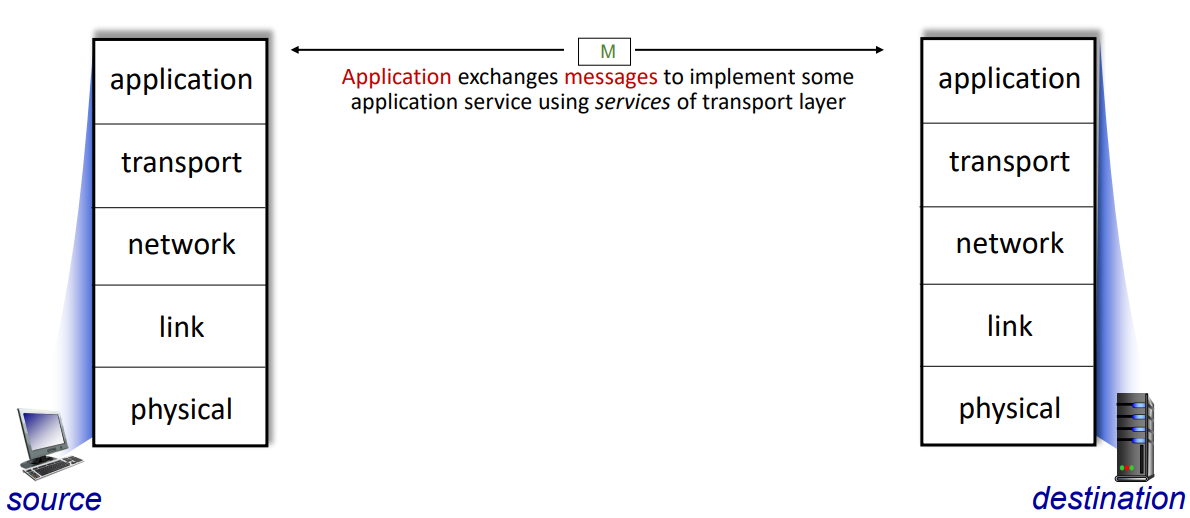
\includegraphics[width =1\linewidth]{Images/25.PNG}
\end{center}
Il messaggio viene quindi passato al livello di trasporto, il quale \textbf{aggiunge un'intestazione (operazione di incapsulamento)} che va ad implementare il servizio a livello di trasporto:
\begin{center}
    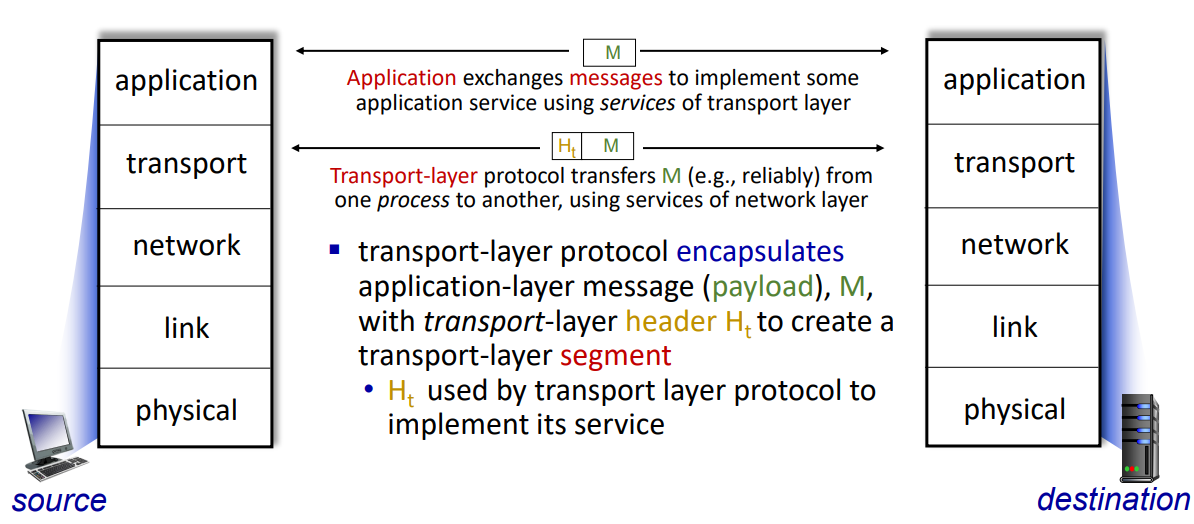
\includegraphics[width =1\linewidth]{Images/26.PNG}
\end{center}
A sua volta, il livello di trasporto usa \textbf{i servizi del livello di rete}, quindi passerò il nuovo \textbf{segmento} al livello di rete, il quale aggiungerà un'ulteriore intestazione:
\begin{center}
    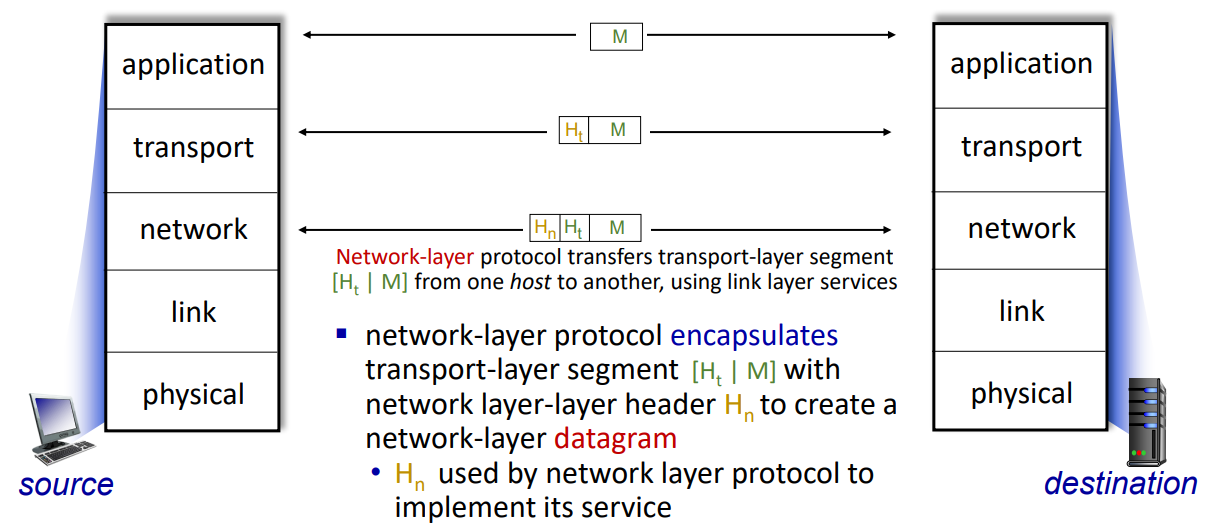
\includegraphics[width =1\linewidth]{Images/27.PNG}
\end{center}
Da notare che a questo livello \textbf{il payload contiene anche l'header del trasporto}, e sarà così anche per le prossime operazioni.
Lo strato di rete si basa sui \textbf{servizi offerti dal livello di collegamento} per implementare i propri, quindi passa il nuovo \textbf{datagramma} ottenuto al livello di collegamento:
\begin{center}
    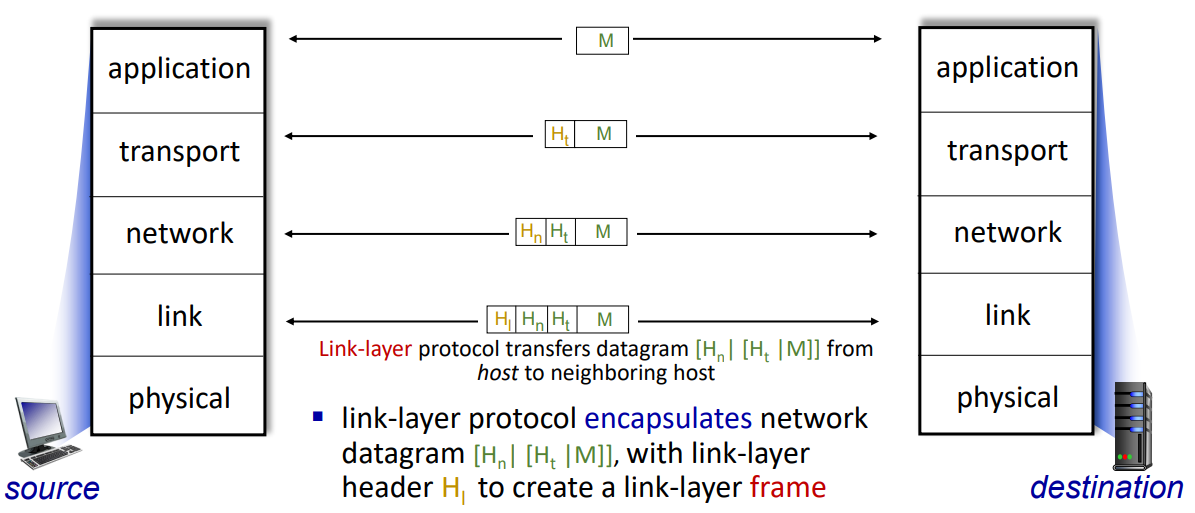
\includegraphics[width =1\linewidth]{Images/28.PNG}
\end{center}
Infine, il pacchetto verrà passato al livello fisico e quindi trasmesso al destinatario.
Come abbiamo già accennato, i pacchetti hanno  nome diverso in strati diversi:
\begin{center}
    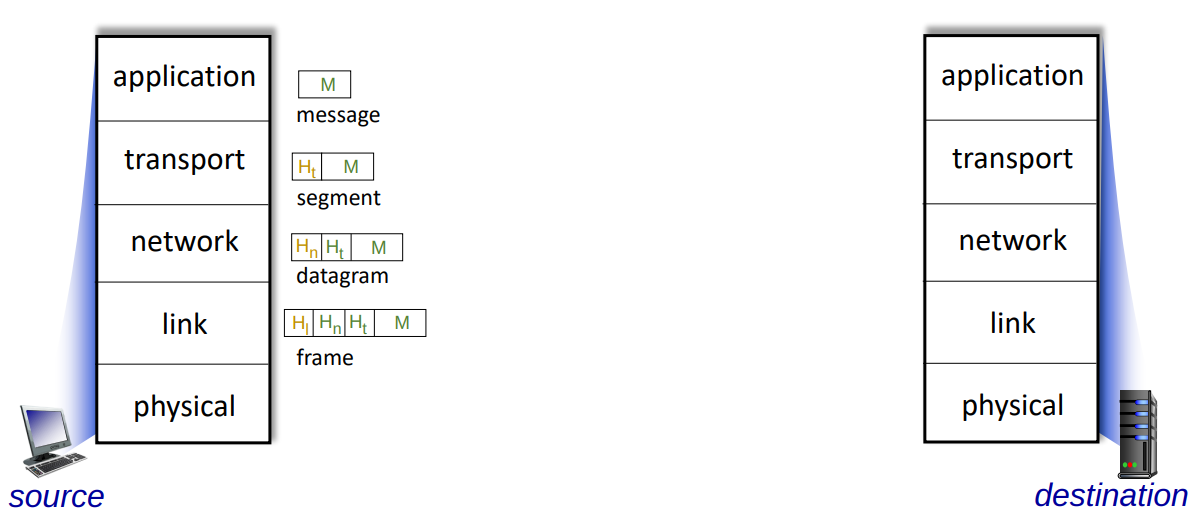
\includegraphics[width =1\linewidth]{Images/29.png}
\end{center}
Man mano che si scende nella pila protocollare, vengono aggiunti nuovi bit di intestazione, i quali servono per \textbf{far funzionare i servizi di rete}.
L'insieme di tutti i bit aggiunti da ogni strato prende il nome di \textbf{overhead} del pacchetto. Poiché il throughput viene misurato \textbf{a livello applicativo},
non si avrà mai, a livello pratico, \textbf{una misura di throughput massima} poiché non vengono contati i bit di overhead. Dopo l'operazione di \textbf{incapsulamento} del messaggio
e di trasmissione su cavo fisico, avviene sul sistema ricevente un'operazione di \textbf{decapsulamento} del messaggio:
\begin{center}
    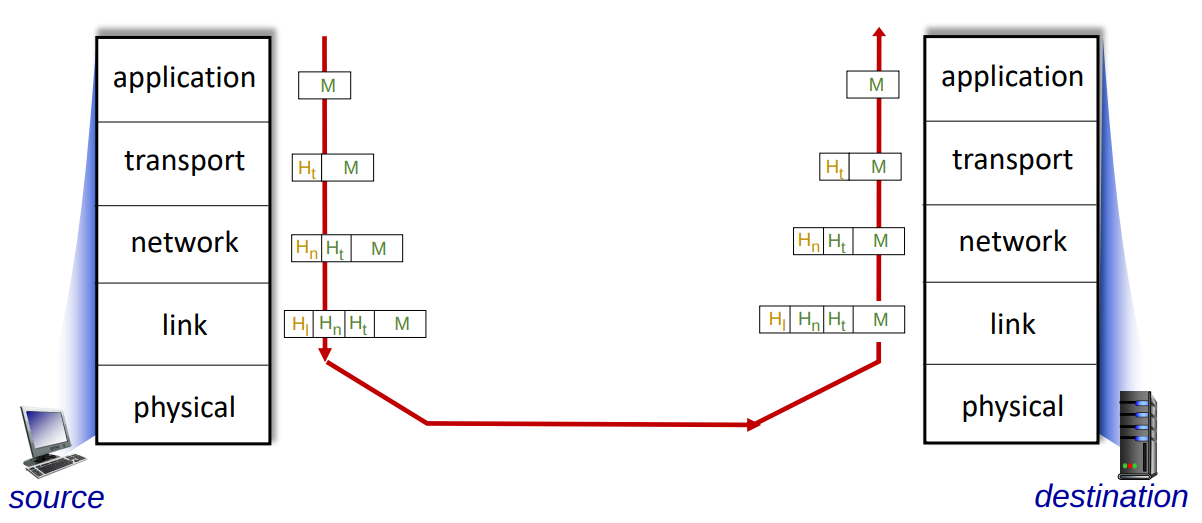
\includegraphics[width =1\linewidth]{Images/30.png}
\end{center}
I sistemi periferici sono sempre in grado di interpretare tutti gli strati della pila protocollare; questo però non è vero per i \textbf{commutatori}, che "parlano" fino al \textbf{livello 2} se sono
degli \textbf{switch} e fino al \textbf{livello 3} se sono dei \textbf{router}:
\begin{center}
    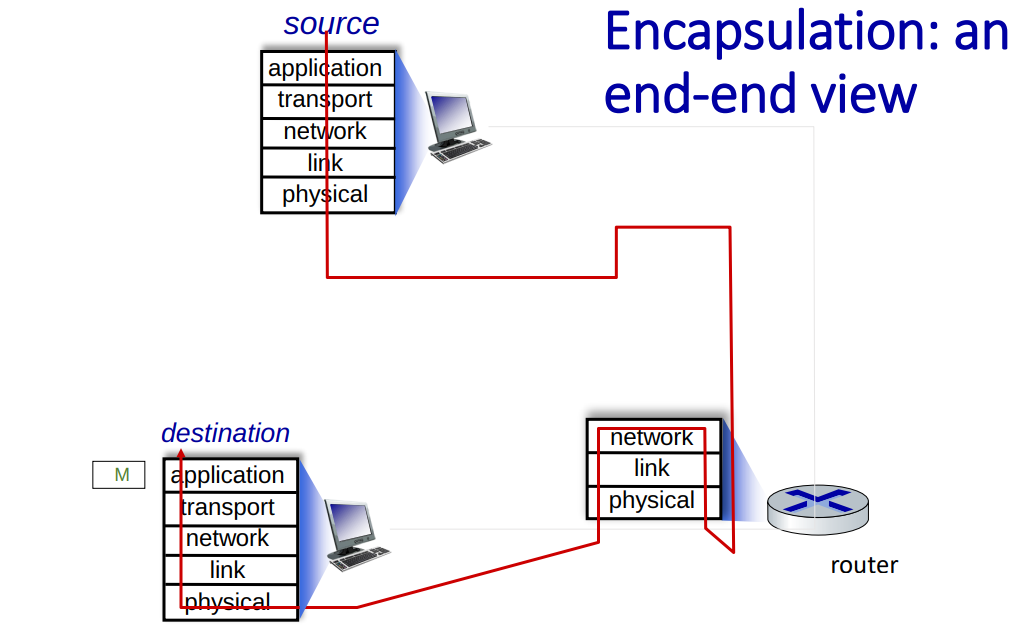
\includegraphics[width = 0.80\linewidth]{Images/31.png}
\end{center}
\section{Strato applicativo: Domain Name System}
Lo strato applicativo ha la funzione di interfacciare e fornire servizi di connettività per i \textbf{processi delle applicazioni}. Il numero
di protocolli presenti in questo strato è altissimo; in questi appunti, tuttavia, ci concentreremo sul protocollo \textbf{DNS}, il quale è una funzionalità chiave di internet, in particolare
se si pensa ad esso come \textbf{fornitore di servizi web}. Quando inseriamo il \textbf{nome} di un sito nel browser, ciò che è avviene è lo scatenamento di un meccanismo che permette al computer
di ottenere \textbf{l'indirizzo IP} (quindi l'indirizzo a livello di rete) associato al server che deve fornire la pagina web richiesta. Per ottenere questo indirizzo IP, non si può pensare di conoscere
ogni indirizzo esistente, quindi è necessario un meccanismo che ci permette di reperirlo: il \textbf{Domain Name System} (DNS). Il DNS permette di effettuare la traduzione dall'\textbf{host name} (i nomi "human readable" dei siti)
all'indirizzo IP del server associato che dovrà fornire al richiedente il contenuto. Come funziona quindi la traduzione? Essa sfrutta la \textbf{gerarchia} di un numero molto elevato di \textbf{server DNS} (che prendono anche il nome di \textbf{name servers}),
i quali andranno a \textbf{risolvere} (tradurre) gli host name in indirizzi IP. Poiché il DNS è un protocollo a livello applicativo, la complessità di questa operazione si trova \textbf{interamente ai confini della rete}.
Il DNS funziona nel seguente modo:
\begin{center}
    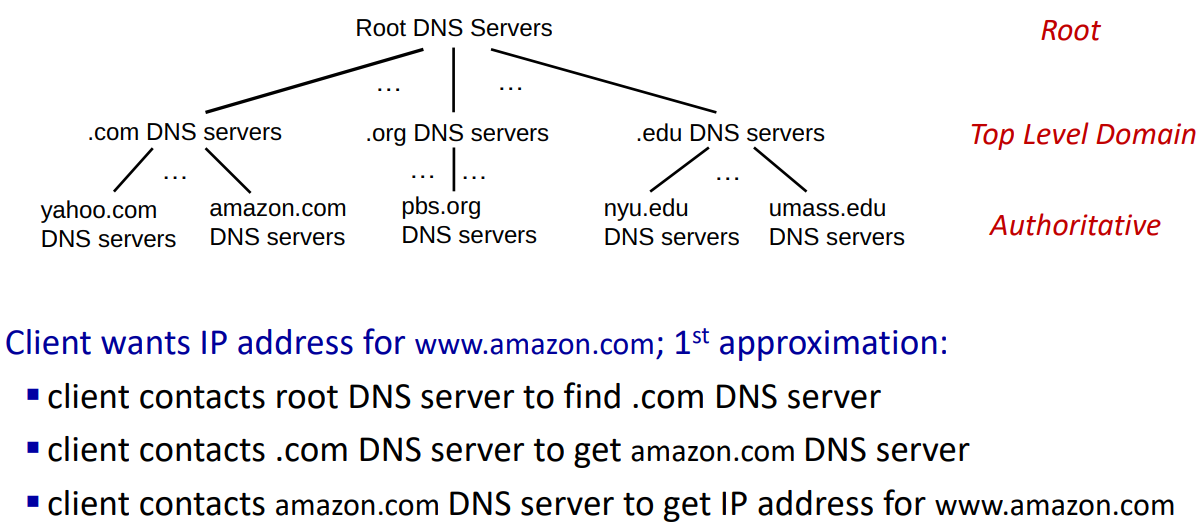
\includegraphics[width = 0.90\linewidth]{Images/32.png}
\end{center}
abbiamo quindi un sistema distribuito che si articola su \textbf{3 livelli}:
\begin{itemize}
    \item \textbf{Root DNS servers}: sono la radice dell'albero gerarchico
    \item \textbf{Top Level Domain (TLD) DNS Servers}: sono responsabili della risoluzione dei \textbf{Top Level Domains}(TLDs); come per esempio .com, .net, .it, ...
    \item \textbf{Authoritative DNS Servers}: Responsabili di risolvere gli indirizzi per i vari domini autoritativi (es. amazon.com, google.com ecc...)
\end{itemize}
Questi 3 livelli collaborano tra loro per risolvere il nome richiesto.
\subsection{Root DNS Servers}
I root DNS server stanno alla radice del sistema DNS e senza la loro esistenza \textbf{è fondamentale per l'esistenza del web}.
In tutto, esistono 13 root name servers "logici", gestiti da \textbf{12 provider differenti}; a loro volta ognuno di questi root dns server è replicato
più volte nel globo. È fondamentale avere repliche dei root name server geograficamente sparse che possono essere acceduti dai vari luogo del mondo.
\begin{center}
    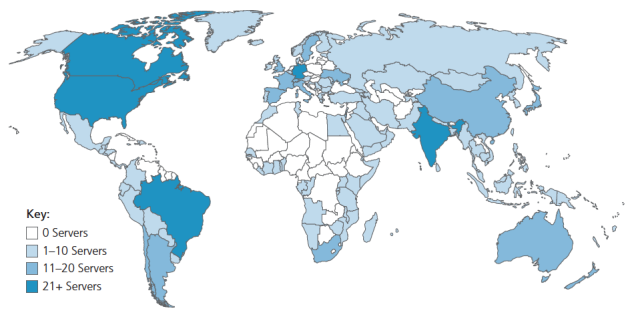
\includegraphics[width = 0.70\linewidth]{Images/33.png}
\end{center}
\subsection{Top Level DNS servers e Authoritative DNS servers}
Ogni TLD DNS server è responsabile per la risoluzione dei TLD, inclusi quelli nazionali (.it, .de. .pl, ...).
I DNS server autoritativi invece è importate specificare che \textbf{possono essere mantenuti dall'organizzazione che detiene il dominio}
oppure \textbf{possono essere mantenuti da un service provider}. Il loro compito è di risolvere le richieste relative a tutte le pagine appartenenti
al loro dominio.
\subsection{Local DNS name servers}
Quando vi è la necessità di contattare il DNS per risolvere un dominio,la prima cosa che viene fatta è contattare il \textbf{DNS server locale}, a cui viene
demandata di fatto questa risoluzione. Il DNS server locale ha un ruolo fondamentale: esistono DNS server locali forniti da ISP, che di solito sono l'opzione di default,
tuttavia un utente può benissimo cambiare il proprio DNS server locale ad uno fornito da un'organizzazione terza. Il DNS server locale tendenzialmente fornisce due servizi:
\begin{itemize}
    \item Mantiene una cache delle associazioni nome-indirizzo IP. Questa cache viene costruita a partire dalle varie richieste dei sistemi terminali e di solito le associazioni
    vengono mantenute per 2 giorni. Il DNS server locale quindi risponderà direttamente alle richieste del client, senza quindi interpellare la gerarchia del DNS, se il nome richiesto è presente
    nella sua cache.
    \item In caso il nome richiesto non sia presente in cache, il DNS server locale procederà ad inoltrare la richiesta alla gerarchia del DNS; una volta ottenuta risposta, procederà a comunicarla al client
\end{itemize}
Ogni richiesta al DNS prende il nome di \textbf{query}.
\subsection{DNS name resolution: Iterated query}
Ci sono due modi per effettuare query al DNS.
Il modo che prende il nome di \textbf{query iterativa} è quello che viene usato più spesso.
In questo metodo, il local DNS server ha \textbf{il maggior carico} dal punto di vista delle richieste da servire.
\begin{center}
    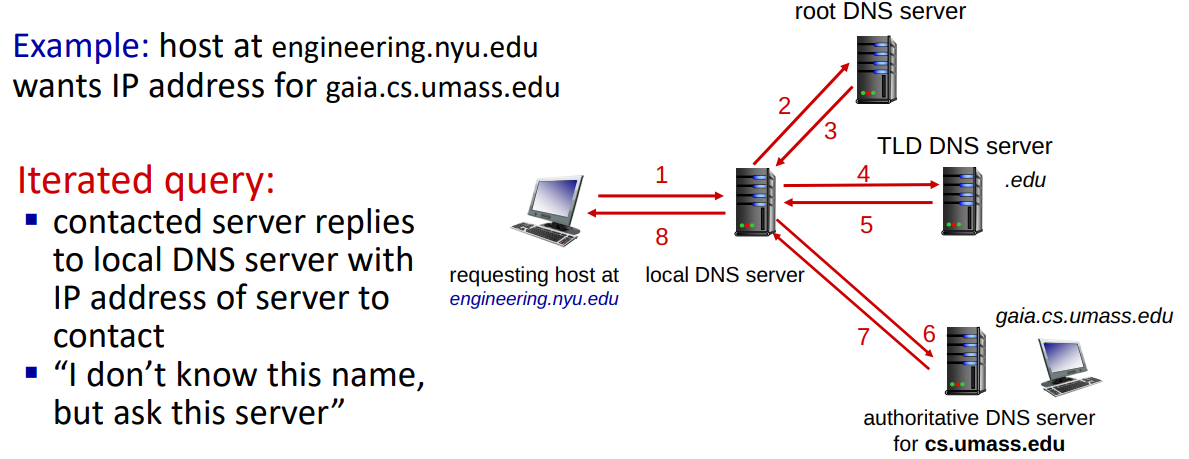
\includegraphics[width = 1\linewidth]{Images/34.png}
\end{center}
\newpage \noindent
Analizziamo nel dettaglio ogni passaggio:
\begin{enumerate}
    \item L'host chiede al DNS server locale di risolvere un certo nome in un indirizzo IP
    \item Il DNS server locale chiede al DNS server root di risolvere il nome
    \item Il DNS server root indica al server DNS server locale quale TLD DNS server può risolvere la sua richiesta
    \item Il DNS server locale chiede al TLD DNS server indicato di risolvere il nome
    \item Il TLD DNS server indica al server DNS locale quale DNS server autoritativo può risolvere la sua richiesta
    \item Il DNS server locale chiede al server DNS autoritativo di risolvere il nome
    \item Il DNS server autoritativo restituisce l'indirizzo IP associato al nome indicato
    \item Il DNS server locale restituisce l'indirizzo IP al client
\end{enumerate}
Ogni passaggio di questo processo è inoltre \textbf{trasparente all'utente}.
\subsection{DNS name resolution: recursive query}
In una query ricorsiva, la risoluzione viene effettuata, in modo gerarchico, dal DNS server di livello superiore.
Il peso delle richieste quindi grava sulla \textbf{struttura gerarchica del DNS}.
\begin{center}
    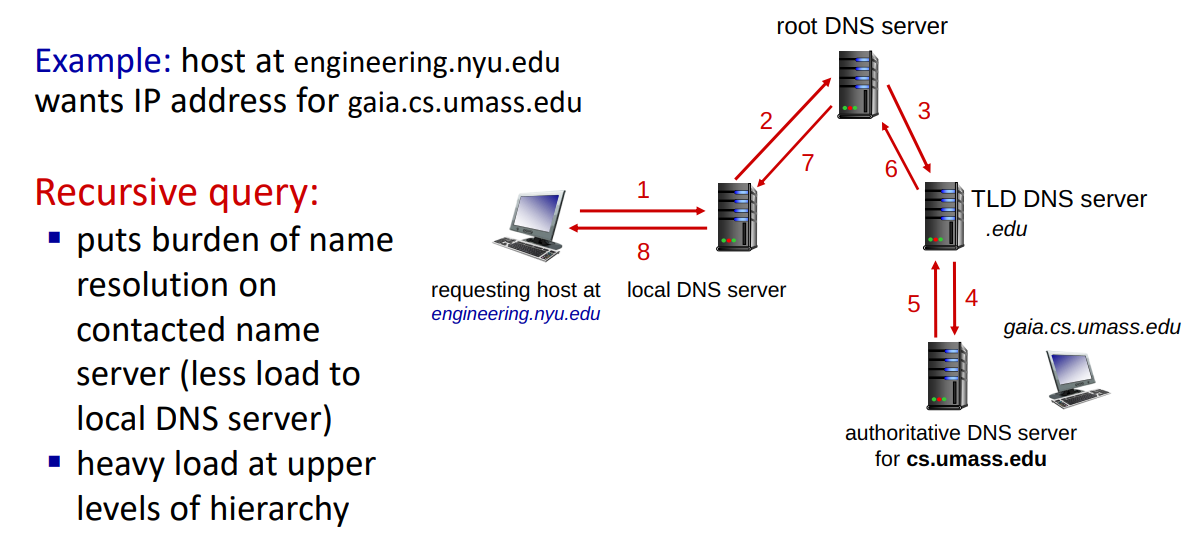
\includegraphics[width = 1\linewidth]{Images/35.png}
\end{center}
Vediamo ogni passo in dettaglio:
\begin{enumerate}
    \item Il client chiede al DNS server locale di risolvere il nome
    \item Il DNS server locale chiede al DNS server di root di risolvere il nome
    \item Il DNS server di root chiede al TLD DNS Server corrispondente di risolvere il nome
    \item Il TLD DNS server chiede al DNS server autoritativo corrispondente di risolvere il nome
    \item Il DNS server autoritativo restituisce l'IP richiesto al TLD DNS server
    \item Il TLD DNS server restituisce la risposta ottenuta al root DNS server
    \item Il root DNS server restituisce la risposta ottenuta al DNS server locale
    \item Il DNS server locale restituisce la risposta ottenuta al client
\end{enumerate}
Solitamente, questo meccanismo non si utilizza poiché tendenzialmente i TLD DNS server, per loro natura, si trovano a gestire
un alta quantità di traffico, quindi un meccanismo di risposta ricorsivo porrebbe ulteriore peso su di essi. Si tende quindi
a cercare di mantenere il peso sui DNS server locali, i quali tendenzialmente gestiscono una quantità di traffico molto minore.


\end{document}